% Options for packages loaded elsewhere
\PassOptionsToPackage{unicode}{hyperref}
\PassOptionsToPackage{hyphens}{url}
\PassOptionsToPackage{dvipsnames,svgnames,x11names}{xcolor}
%
\documentclass[
  letterpaper,
  DIV=11,
  numbers=noendperiod]{scrartcl}

\usepackage{amsmath,amssymb}
\usepackage{iftex}
\ifPDFTeX
  \usepackage[T1]{fontenc}
  \usepackage[utf8]{inputenc}
  \usepackage{textcomp} % provide euro and other symbols
\else % if luatex or xetex
  \usepackage{unicode-math}
  \defaultfontfeatures{Scale=MatchLowercase}
  \defaultfontfeatures[\rmfamily]{Ligatures=TeX,Scale=1}
\fi
\usepackage{lmodern}
\ifPDFTeX\else  
    % xetex/luatex font selection
\fi
% Use upquote if available, for straight quotes in verbatim environments
\IfFileExists{upquote.sty}{\usepackage{upquote}}{}
\IfFileExists{microtype.sty}{% use microtype if available
  \usepackage[]{microtype}
  \UseMicrotypeSet[protrusion]{basicmath} % disable protrusion for tt fonts
}{}
\makeatletter
\@ifundefined{KOMAClassName}{% if non-KOMA class
  \IfFileExists{parskip.sty}{%
    \usepackage{parskip}
  }{% else
    \setlength{\parindent}{0pt}
    \setlength{\parskip}{6pt plus 2pt minus 1pt}}
}{% if KOMA class
  \KOMAoptions{parskip=half}}
\makeatother
\usepackage{xcolor}
\setlength{\emergencystretch}{3em} % prevent overfull lines
\setcounter{secnumdepth}{-\maxdimen} % remove section numbering
% Make \paragraph and \subparagraph free-standing
\ifx\paragraph\undefined\else
  \let\oldparagraph\paragraph
  \renewcommand{\paragraph}[1]{\oldparagraph{#1}\mbox{}}
\fi
\ifx\subparagraph\undefined\else
  \let\oldsubparagraph\subparagraph
  \renewcommand{\subparagraph}[1]{\oldsubparagraph{#1}\mbox{}}
\fi

\usepackage{color}
\usepackage{fancyvrb}
\newcommand{\VerbBar}{|}
\newcommand{\VERB}{\Verb[commandchars=\\\{\}]}
\DefineVerbatimEnvironment{Highlighting}{Verbatim}{commandchars=\\\{\}}
% Add ',fontsize=\small' for more characters per line
\usepackage{framed}
\definecolor{shadecolor}{RGB}{241,243,245}
\newenvironment{Shaded}{\begin{snugshade}}{\end{snugshade}}
\newcommand{\AlertTok}[1]{\textcolor[rgb]{0.68,0.00,0.00}{#1}}
\newcommand{\AnnotationTok}[1]{\textcolor[rgb]{0.37,0.37,0.37}{#1}}
\newcommand{\AttributeTok}[1]{\textcolor[rgb]{0.40,0.45,0.13}{#1}}
\newcommand{\BaseNTok}[1]{\textcolor[rgb]{0.68,0.00,0.00}{#1}}
\newcommand{\BuiltInTok}[1]{\textcolor[rgb]{0.00,0.23,0.31}{#1}}
\newcommand{\CharTok}[1]{\textcolor[rgb]{0.13,0.47,0.30}{#1}}
\newcommand{\CommentTok}[1]{\textcolor[rgb]{0.37,0.37,0.37}{#1}}
\newcommand{\CommentVarTok}[1]{\textcolor[rgb]{0.37,0.37,0.37}{\textit{#1}}}
\newcommand{\ConstantTok}[1]{\textcolor[rgb]{0.56,0.35,0.01}{#1}}
\newcommand{\ControlFlowTok}[1]{\textcolor[rgb]{0.00,0.23,0.31}{#1}}
\newcommand{\DataTypeTok}[1]{\textcolor[rgb]{0.68,0.00,0.00}{#1}}
\newcommand{\DecValTok}[1]{\textcolor[rgb]{0.68,0.00,0.00}{#1}}
\newcommand{\DocumentationTok}[1]{\textcolor[rgb]{0.37,0.37,0.37}{\textit{#1}}}
\newcommand{\ErrorTok}[1]{\textcolor[rgb]{0.68,0.00,0.00}{#1}}
\newcommand{\ExtensionTok}[1]{\textcolor[rgb]{0.00,0.23,0.31}{#1}}
\newcommand{\FloatTok}[1]{\textcolor[rgb]{0.68,0.00,0.00}{#1}}
\newcommand{\FunctionTok}[1]{\textcolor[rgb]{0.28,0.35,0.67}{#1}}
\newcommand{\ImportTok}[1]{\textcolor[rgb]{0.00,0.46,0.62}{#1}}
\newcommand{\InformationTok}[1]{\textcolor[rgb]{0.37,0.37,0.37}{#1}}
\newcommand{\KeywordTok}[1]{\textcolor[rgb]{0.00,0.23,0.31}{#1}}
\newcommand{\NormalTok}[1]{\textcolor[rgb]{0.00,0.23,0.31}{#1}}
\newcommand{\OperatorTok}[1]{\textcolor[rgb]{0.37,0.37,0.37}{#1}}
\newcommand{\OtherTok}[1]{\textcolor[rgb]{0.00,0.23,0.31}{#1}}
\newcommand{\PreprocessorTok}[1]{\textcolor[rgb]{0.68,0.00,0.00}{#1}}
\newcommand{\RegionMarkerTok}[1]{\textcolor[rgb]{0.00,0.23,0.31}{#1}}
\newcommand{\SpecialCharTok}[1]{\textcolor[rgb]{0.37,0.37,0.37}{#1}}
\newcommand{\SpecialStringTok}[1]{\textcolor[rgb]{0.13,0.47,0.30}{#1}}
\newcommand{\StringTok}[1]{\textcolor[rgb]{0.13,0.47,0.30}{#1}}
\newcommand{\VariableTok}[1]{\textcolor[rgb]{0.07,0.07,0.07}{#1}}
\newcommand{\VerbatimStringTok}[1]{\textcolor[rgb]{0.13,0.47,0.30}{#1}}
\newcommand{\WarningTok}[1]{\textcolor[rgb]{0.37,0.37,0.37}{\textit{#1}}}

\providecommand{\tightlist}{%
  \setlength{\itemsep}{0pt}\setlength{\parskip}{0pt}}\usepackage{longtable,booktabs,array}
\usepackage{calc} % for calculating minipage widths
% Correct order of tables after \paragraph or \subparagraph
\usepackage{etoolbox}
\makeatletter
\patchcmd\longtable{\par}{\if@noskipsec\mbox{}\fi\par}{}{}
\makeatother
% Allow footnotes in longtable head/foot
\IfFileExists{footnotehyper.sty}{\usepackage{footnotehyper}}{\usepackage{footnote}}
\makesavenoteenv{longtable}
\usepackage{graphicx}
\makeatletter
\def\maxwidth{\ifdim\Gin@nat@width>\linewidth\linewidth\else\Gin@nat@width\fi}
\def\maxheight{\ifdim\Gin@nat@height>\textheight\textheight\else\Gin@nat@height\fi}
\makeatother
% Scale images if necessary, so that they will not overflow the page
% margins by default, and it is still possible to overwrite the defaults
% using explicit options in \includegraphics[width, height, ...]{}
\setkeys{Gin}{width=\maxwidth,height=\maxheight,keepaspectratio}
% Set default figure placement to htbp
\makeatletter
\def\fps@figure{htbp}
\makeatother
\newlength{\cslhangindent}
\setlength{\cslhangindent}{1.5em}
\newlength{\csllabelwidth}
\setlength{\csllabelwidth}{3em}
\newlength{\cslentryspacingunit} % times entry-spacing
\setlength{\cslentryspacingunit}{\parskip}
\newenvironment{CSLReferences}[2] % #1 hanging-ident, #2 entry spacing
 {% don't indent paragraphs
  \setlength{\parindent}{0pt}
  % turn on hanging indent if param 1 is 1
  \ifodd #1
  \let\oldpar\par
  \def\par{\hangindent=\cslhangindent\oldpar}
  \fi
  % set entry spacing
  \setlength{\parskip}{#2\cslentryspacingunit}
 }%
 {}
\usepackage{calc}
\newcommand{\CSLBlock}[1]{#1\hfill\break}
\newcommand{\CSLLeftMargin}[1]{\parbox[t]{\csllabelwidth}{#1}}
\newcommand{\CSLRightInline}[1]{\parbox[t]{\linewidth - \csllabelwidth}{#1}\break}
\newcommand{\CSLIndent}[1]{\hspace{\cslhangindent}#1}

\KOMAoption{captions}{tableheading}
\makeatletter
\makeatother
\makeatletter
\makeatother
\makeatletter
\@ifpackageloaded{caption}{}{\usepackage{caption}}
\AtBeginDocument{%
\ifdefined\contentsname
  \renewcommand*\contentsname{Table of contents}
\else
  \newcommand\contentsname{Table of contents}
\fi
\ifdefined\listfigurename
  \renewcommand*\listfigurename{List of Figures}
\else
  \newcommand\listfigurename{List of Figures}
\fi
\ifdefined\listtablename
  \renewcommand*\listtablename{List of Tables}
\else
  \newcommand\listtablename{List of Tables}
\fi
\ifdefined\figurename
  \renewcommand*\figurename{Figure}
\else
  \newcommand\figurename{Figure}
\fi
\ifdefined\tablename
  \renewcommand*\tablename{Table}
\else
  \newcommand\tablename{Table}
\fi
}
\@ifpackageloaded{float}{}{\usepackage{float}}
\floatstyle{ruled}
\@ifundefined{c@chapter}{\newfloat{codelisting}{h}{lop}}{\newfloat{codelisting}{h}{lop}[chapter]}
\floatname{codelisting}{Listing}
\newcommand*\listoflistings{\listof{codelisting}{List of Listings}}
\makeatother
\makeatletter
\@ifpackageloaded{caption}{}{\usepackage{caption}}
\@ifpackageloaded{subcaption}{}{\usepackage{subcaption}}
\makeatother
\makeatletter
\@ifpackageloaded{tcolorbox}{}{\usepackage[skins,breakable]{tcolorbox}}
\makeatother
\makeatletter
\@ifundefined{shadecolor}{\definecolor{shadecolor}{rgb}{.97, .97, .97}}
\makeatother
\makeatletter
\makeatother
\makeatletter
\makeatother
\ifLuaTeX
  \usepackage{selnolig}  % disable illegal ligatures
\fi
\IfFileExists{bookmark.sty}{\usepackage{bookmark}}{\usepackage{hyperref}}
\IfFileExists{xurl.sty}{\usepackage{xurl}}{} % add URL line breaks if available
\urlstyle{same} % disable monospaced font for URLs
\hypersetup{
  pdftitle={FYS-STK Exercises week 38},
  colorlinks=true,
  linkcolor={blue},
  filecolor={Maroon},
  citecolor={Blue},
  urlcolor={Blue},
  pdfcreator={LaTeX via pandoc}}

\title{FYS-STK Exercises week 38}
\author{}
\date{}

\begin{document}
\maketitle
\ifdefined\Shaded\renewenvironment{Shaded}{\begin{tcolorbox}[enhanced, sharp corners, breakable, frame hidden, interior hidden, borderline west={3pt}{0pt}{shadecolor}, boxrule=0pt]}{\end{tcolorbox}}\fi

We generate a data set of n=100 similar to that from week 36 to
investigate the bias-variance tradeoff. The input data has polynomial
features of degree 1 to 15, i.e., increasing complexity. Then we run an
ordinary least squares (OLS) model on the data for with 100 resamplings
for each polynomial degree, and estimate error, bias and variance of our
model.

The following code is mostly made from scratch, with the bias, variance
and mse calculations taken from the course book (Hjort-Jensen 2021).

\begin{Shaded}
\begin{Highlighting}[]
\ImportTok{import}\NormalTok{ numpy }\ImportTok{as}\NormalTok{ np}
\ImportTok{import}\NormalTok{ matplotlib.pyplot }\ImportTok{as}\NormalTok{ plt}
\ImportTok{from}\NormalTok{ sklearn.utils }\ImportTok{import}\NormalTok{ resample}
\ImportTok{from}\NormalTok{ sklearn.linear\_model }\ImportTok{import}\NormalTok{ LinearRegression}
\ImportTok{from}\NormalTok{ sklearn.model\_selection }\ImportTok{import}\NormalTok{ train\_test\_split}

\KeywordTok{def}\NormalTok{ design\_poly\_n(x, n):}
\NormalTok{    X }\OperatorTok{=}\NormalTok{ np.zeros((}\BuiltInTok{len}\NormalTok{(x), n))}
\NormalTok{    X[:,}\DecValTok{0}\NormalTok{] }\OperatorTok{=} \DecValTok{1}
    \ControlFlowTok{for}\NormalTok{ i }\KeywordTok{in} \BuiltInTok{range}\NormalTok{(}\DecValTok{1}\NormalTok{, n):}
\NormalTok{        X[:,i] }\OperatorTok{=}\NormalTok{ (x}\OperatorTok{**}\NormalTok{i).T}
    \ControlFlowTok{return}\NormalTok{ X}

\NormalTok{np.random.seed(}\DecValTok{3490}\NormalTok{)}
\NormalTok{n }\OperatorTok{=} \DecValTok{100}
\CommentTok{\# Make data set.}
\NormalTok{x }\OperatorTok{=}\NormalTok{ np.linspace(}\OperatorTok{{-}}\DecValTok{3}\NormalTok{, }\DecValTok{3}\NormalTok{, n).reshape(}\OperatorTok{{-}}\DecValTok{1}\NormalTok{, }\DecValTok{1}\NormalTok{)}
\NormalTok{y }\OperatorTok{=}\NormalTok{ np.exp(}\OperatorTok{{-}}\NormalTok{x}\OperatorTok{**}\DecValTok{2}\NormalTok{) }\OperatorTok{+} \FloatTok{1.5} \OperatorTok{*}\NormalTok{ np.exp(}\OperatorTok{{-}}\NormalTok{(x}\OperatorTok{{-}}\DecValTok{2}\NormalTok{)}\OperatorTok{**}\DecValTok{2}\NormalTok{)}\OperatorTok{+}\NormalTok{ np.random.normal(}\DecValTok{0}\NormalTok{, }\FloatTok{0.1}\NormalTok{, x.shape)}

\NormalTok{np.random.seed(}\DecValTok{5}\NormalTok{)}
\NormalTok{npoly }\OperatorTok{=} \DecValTok{15}
\NormalTok{X }\OperatorTok{=}\NormalTok{ design\_poly\_n(x, npoly }\OperatorTok{+} \DecValTok{1}\NormalTok{)[:,}\DecValTok{1}\NormalTok{:]}
\NormalTok{X\_train, X\_test, y\_train, y\_test }\OperatorTok{=}\NormalTok{ train\_test\_split(X, y, test\_size}\OperatorTok{=}\FloatTok{0.2}\NormalTok{)}

\NormalTok{polys }\OperatorTok{=}\NormalTok{ np.arange(npoly) }\OperatorTok{+} \DecValTok{1}
\NormalTok{mse }\OperatorTok{=}\NormalTok{ np.zeros(npoly)}
\NormalTok{bias }\OperatorTok{=}\NormalTok{ np.zeros(npoly)}
\NormalTok{variance }\OperatorTok{=}\NormalTok{ np.zeros(npoly)}
\NormalTok{nbootstraps }\OperatorTok{=} \DecValTok{100}

\CommentTok{\# fit models with resampling}

\ControlFlowTok{for}\NormalTok{ i }\KeywordTok{in}\NormalTok{ polys:}
\NormalTok{    y\_pred }\OperatorTok{=}\NormalTok{ np.zeros((y\_test.shape[}\DecValTok{0}\NormalTok{], nbootstraps))}
\NormalTok{    X\_train\_deg }\OperatorTok{=}\NormalTok{ X\_train[:,:i]}
    \ControlFlowTok{for}\NormalTok{ j }\KeywordTok{in} \BuiltInTok{range}\NormalTok{(nbootstraps):}
\NormalTok{        x\_tmp, y\_tmp }\OperatorTok{=}\NormalTok{ resample(X\_train\_deg, y\_train)}
\NormalTok{        lr }\OperatorTok{=}\NormalTok{ LinearRegression(fit\_intercept}\OperatorTok{=}\VariableTok{False}\NormalTok{).fit(x\_tmp, y\_tmp)}
\NormalTok{        y\_pred[:,j] }\OperatorTok{=}\NormalTok{ lr.predict(X\_test[:,:i]).ravel()}
\NormalTok{    mse[i}\OperatorTok{{-}}\DecValTok{1}\NormalTok{] }\OperatorTok{=}\NormalTok{ np.mean( np.mean((y\_test }\OperatorTok{{-}}\NormalTok{ y\_pred)}\OperatorTok{**}\DecValTok{2}\NormalTok{, axis }\OperatorTok{=} \DecValTok{1}\NormalTok{, keepdims }\OperatorTok{=} \VariableTok{True}\NormalTok{) )}
\NormalTok{    bias[i}\OperatorTok{{-}}\DecValTok{1}\NormalTok{] }\OperatorTok{=}\NormalTok{ np.mean((y\_test }\OperatorTok{{-}}\NormalTok{ np.mean(y\_pred, axis }\OperatorTok{=} \DecValTok{1}\NormalTok{, keepdims }\OperatorTok{=} \VariableTok{True}\NormalTok{))}\OperatorTok{**}\DecValTok{2}\NormalTok{)}
\NormalTok{    variance[i}\OperatorTok{{-}}\DecValTok{1}\NormalTok{] }\OperatorTok{=}\NormalTok{ np.mean(np.var(y\_pred, axis }\OperatorTok{=} \DecValTok{0}\NormalTok{, keepdims }\OperatorTok{=} \VariableTok{True}\NormalTok{))}

\NormalTok{plt.clf()}
\NormalTok{plt.plot(polys, mse, label }\OperatorTok{=} \StringTok{"Error"}\NormalTok{)}
\NormalTok{plt.plot(polys, bias, label }\OperatorTok{=} \StringTok{"Bias"}\NormalTok{)}
\NormalTok{plt.plot(polys, variance, label }\OperatorTok{=} \StringTok{"Variance"}\NormalTok{)}
\NormalTok{plt.legend()}
\NormalTok{plt.xlabel(}\StringTok{"Polynomial degrees"}\NormalTok{)}
\NormalTok{plt.ylabel(}\StringTok{"Value"}\NormalTok{)}
\NormalTok{plt.show()}
\end{Highlighting}
\end{Shaded}

\begin{figure}[H]

{\centering 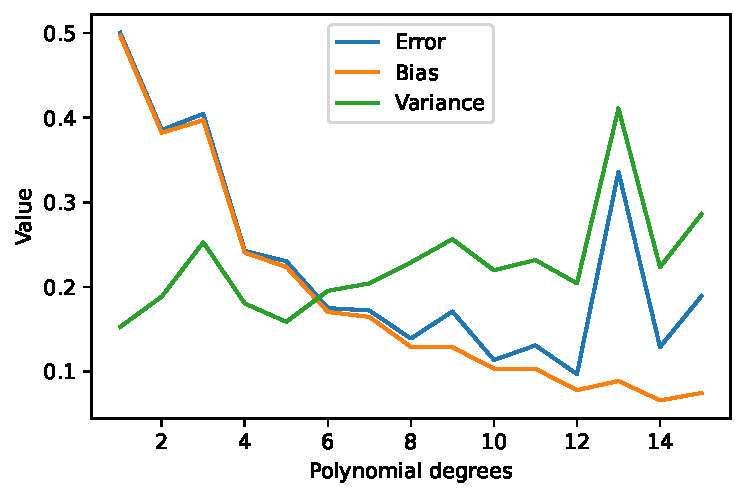
\includegraphics{w38-exercises_files/figure-pdf/fig-bias-var-output-1.pdf}

}

\caption{\label{fig-bias-var}Error, bias and variance for a polynomial
fit up to degree 15. The training data was bootstrapped with 100
resamplings per polynomial degree.}

\end{figure}

From Figure~\ref{fig-bias-var} we see that bias decreases with model
complexity while variance increases, and that the error has some optimal
complexity around degree 10-12. A more complex model will generally have
lower bias, but is very sensitive to changes in the data used to fit the
model, resulting in a higher model variance.

\hypertarget{refs}{}
\begin{CSLReferences}{1}{0}
\leavevmode\vadjust pre{\hypertarget{ref-fys_stk_book}{}}%
Hjort-Jensen, Morten. 2021. \emph{Applied Data Analysis and Machine
Learning}. Jupyter Notebook.

\end{CSLReferences}



\end{document}
